%!TEX program = lualatex
\documentclass[bachelorarbeit,grey,english]{mas-thesis-sections}				% Available options:
															% masterarbeit, bachelorarbeit, dissertation,
															% masterprojekt, bachelorprojekt, seminararbeit,
															% fallstudie, grey (für Graustufen), english

\author{Autorname}
\title{Titel der Arbeit}
\supervisor{Univ.-Prof.~Dipl.-Ing.~Dr.~Betreuer~Name}	% ~ for nicer spaces
\reviewerA{Univ.-Prof.~Dr.~Tobias~Hoßfeld}
\reviewerB{Gutachter~B}
\degreecourse{Angewandte Informatik - Network Engineering}
\location{Essen}
%\linespread{1.25}										% Line spread (default is 1.25)
\handoverdate{13.03.2015}

%%%%%%%%%%%%%% 
%TODO:

%\usepackage{array}


%% load bibs
\addbibresource{bibliography/bibliography.bib}
%\addbibresource{bibliography/more-bibliography.bib}



%\input{components/info}

%\DeclareBibliographyCategory{ownpub}

%%%%%%%%%%%%%%%%%%%%%%%%%%%%%%%%%%%%%%%%%%%%%%%%%%%%%%%%%%%%%%%%%%%%%%%%%%%%%%%%
\begin{document}

\maketitle				% Title Page

\cleardoublepage

\pagenumbering{Roman}
\tableofcontents		% Table of Contents

\cleardoublepage

\listofillustrations	% List of Figures and List of Tables


\cleardoublepage

\pagenumbering{arabic}
\setcounter{page}{1}

\chapter{Introduction}	% Remove if not dissertation or masterarbeit

\section{Abstract}

This document is a short example of how to use this template to write your own thesis. It gives a brief summary of the most important aspects and options that define this template.

\newpage


\section{General}

There are 2 differnt class files available: mas-thesis-sections and mas-thesis-chapters. Use the first if you plan to write a short thesis like a Bachelor Project or a Case Study and ignores chapters for the most past. The latter is better suited for a Master Thesis or Dissertation because it allows you to divide your thesis better. But nothing stops you to devide your Bachelor Thesis in chapters if you think that it will fit.

\newpage


\section{Sections}

This is an example of a numbered section. The section number increases automatically and does not need to be stated. To use a unnumbered section, just use {\tt \textbackslash section* \{Name of unnumbered section\}}. A section can be divided by multiple subsections.

\subsection{Subsections}

This is a numerated {\tt \textbackslash subsection}. There is also a {\tt \textbackslash subsubsection} command. To create an unnumbered subsection, just add * like needed for sections.

\newpage

\section{Imports}

Large thesis like master thesis and dissertations often get very confusing when written in single document. You can import other .tex files with the {\tt \textbackslash include\{other-latex-file.tex\}} command. The formatting will be taken from the master file and the sections, figures, tables, footnotes, citations, etc. are integrated in the context of the master file.

\newpage


\section{Tables and Figures}

In \LaTeX\ you can use tables and figures which will be automatically added to the List of Tables and List of Figures after the Table of Contents.

\subsection{Tables}

\begin{table}[ht]
\begin{center}
	\begin{tabular}{ l | c | r }
		1 & 2 & 3 \\
		\hline
		4 & 5 & 6 \\
		7 & 8 & 9 \\
	\end{tabular}
	\caption{Example of a table}
	\label{table:1}
\end{center}
\end{table}

\subsection{Figures}

Figures should be vector graphics where possible. \LaTeX can parse PDF and EPS out of the box but SVG can also be used with the svg package. If no vector graphics are available and you need to include raster graphics like JPEG, PNG, or BMP, make sure you have a high resolution and high DPI image. Note that the resulting PDF file can be very large when using a lot of raster graphics.

\begin{figure}[ht]
	\centering
	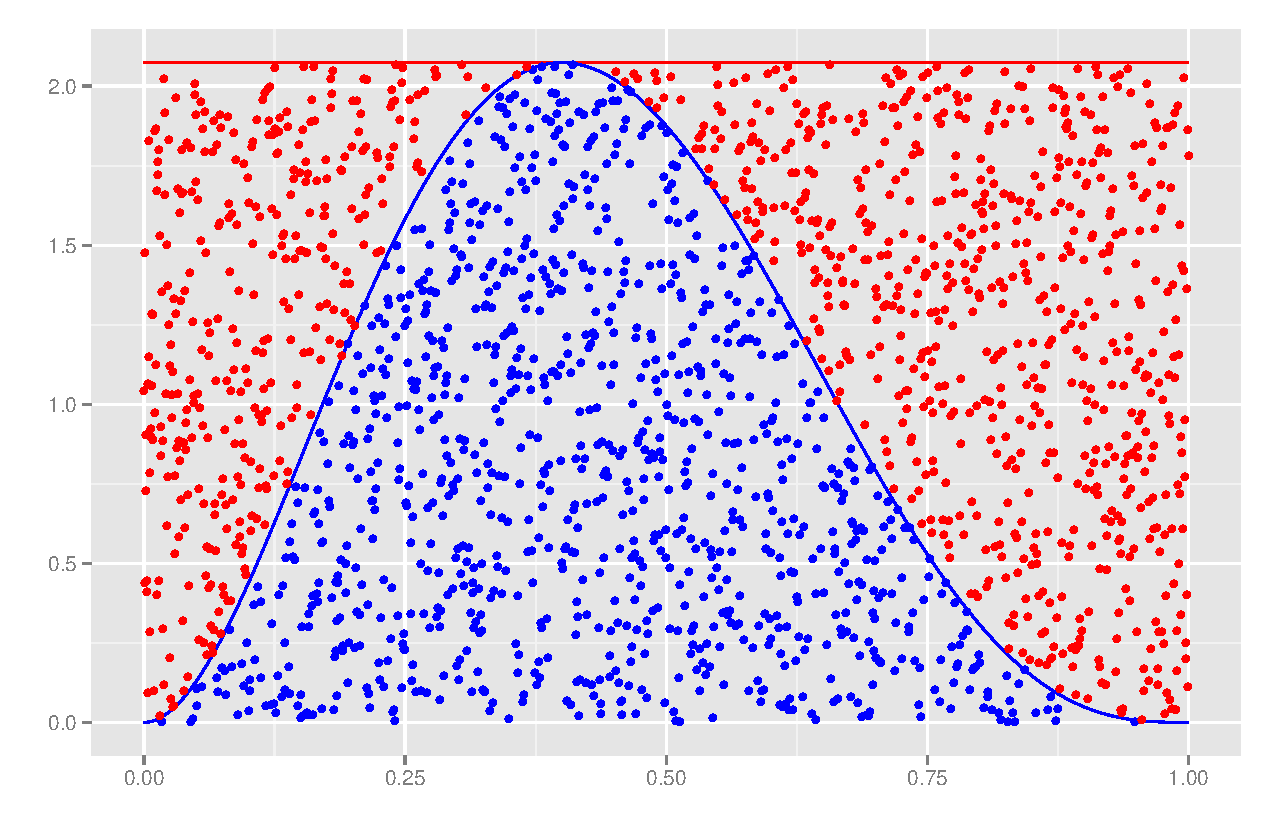
\includegraphics[height=5.1cm]{graphics/demo-graphic.pdf}
	\caption{Example of an imported PDF graphic}
	\label{figure:1}
\end{figure}

\newpage

\section{Bib\TeX\ and Footnotes}

Every thesis contains references. With Bib\TeX\footnote{\url{http://www.bibtex.org}} you can easily define them in one or more files and load them with \LaTeX\ and cite them at any time.\cite{exampleBook}
\cleardoublepage

\printbibliography

\makelicensepageCCBYSA


% \input{components/license.tex}
% \input{components/toc.tex}
% \input{components/indices.tex}
% \input{components/quote.tex}
% \input{components/abstract.tex}
% \input{components/acknowledgments.tex}

%\newpage
%\listoftodos


%%%%%%%%%%%%%%%%%%%%%%%%%%%%%%%%%%%%%%%%%%%%%%%%%%%%%%%%%%%%%%%%%%%%%%%%%%%%%%%%
% \cleardoublepage
% \pagenumbering{arabic}

% \subimport{chapters/01-intro/}{introduction}
% \subimport{chapters/04-mobilenets/}{mobilenetworks}
% \subimport{chapters/041-mobilenetsmeasuring/}{mobilenetworkevaluation}
% \subimport{chapters/03-streaming/}{streaming}
% \subimport{chapters/05-mobilestreaming/}{mobilestreaming}
% \subimport{chapters/06-mobilestreamingmeasurements/}{measurements}
% \subimport{chapters/99-conclusion/}{conclusion}


%%%%%%%%%%%%%%%%%%%%%%%%%%%%%%%%%%%%%%%%%%%%%%%%%%%%%%%%%%%%%%%%%%%%%%%%%%%%%%%%

% \input{components/vita.tex}

% \addtocategory{ownpub}{metzger2012research, oechsner2009pushing,metzger2014lossmodel,raf2013sensorium, cs3516, metzger2014jcnc, rafetseder2011explyt, 6229739, metzger2011delivery, cs3518}
% \nocite{oechsner2009pushing,metzger2014lossmodel,raf2013sensorium,cs3516} % temporary import of otherwise unreferences own publications


% \defbibnote{ownpubdisclaimer}{Parts of the research conducted in this thesis is based on these already published publications. }
% \printbibliography[title=Own Publications, category=ownpub, heading=bibintoc, prenote=ownpubdisclaimer]


% %\section*{Own Publications}
% %\addcontentsline{toc}{chapter}{Own Publications}%

% %\printbibliography[category=ownpub]

% \input{components/sourcecode.tex}
% %\printbibliography[notkeyword=ownpub, heading=bibintoc]
% \printbibliography[notcategory=ownpub, heading=bibintoc]
\end{document}
